\section{Description of the hardware structure and functionality}

In this section the different components of the hardware will be listed, described and explained.\


\section{Hardware diagram}
\begin{figure}[!ht]
	\centering
	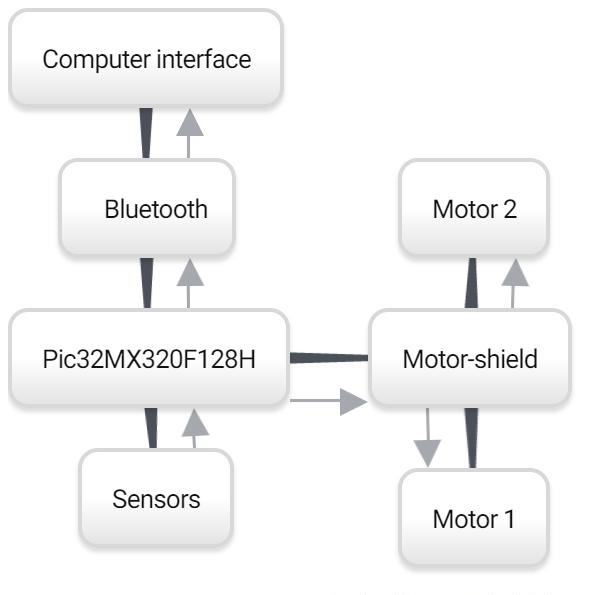
\includegraphics[width=0.7\textwidth]{figures/hardwareDIA.jpg}
	\caption{\text{Hardware diagram with arrows}}
	\label{Hardware diagram}
\end{figure}



The micro controller is connected to the motor-shield.\ The motor-shield is then connected to the two motors, called motor 1 and motor 2 and is powering both motors.\ The micro controller is receiving data from the 3 sensor sets; the ultrasound sensors, infrared light-sensors and the tachometer sensor.\ The micro controller then receives the data from the sensors and sends it further to the Bluetooth transceiver and then the Bluetooth transceiver will send it to the interface. \\ \\

\section{Sensors and sensor concept}

TBD: Find out why this doesn't show up in build...

The robot will utilize two sets on sensors - one set of QRE1113 sensors, which will be used for line-following capabilities, they are fastened towards the end of the robot, and will give the robot a way to detect what surface it is about to enter.\\
The second is a hybrid set of ultrasound and infrared sensors. These will be working together to make the robot able to navigate open spaces more precisely, since infrared and ultrasound sensors work the best under different circumstances. This will end up as a product which is more optimized for usage in situations that would not be ideal for one of the other, since the hybrid design will leverage shortcomings of a given sensor method.\\

\subsection{Ultrasound sensor - HC-SR04}
When a robot should be able avoid obstacles it will need a device to inform the robot where it's position is compared to the obstacle. This is where an ultrasound sensor plays an important role. For this task the HC sr04 has been picked.\\

\begin{figure}[!ht]
	\centering
	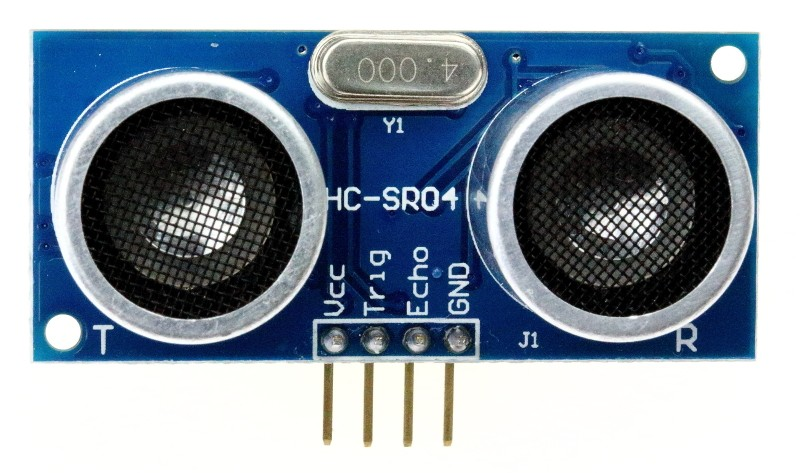
\includegraphics[width=0.7\textwidth]{figures/hc04.jpg}
	\caption{\text{The HC-SR04 ultrasound sensor}}
	\label{Hardware diagram}
\end{figure}


The way the ultrasound sensor works is by emitting acoustic waves and then waits for the waves to reflect back to the sensor. The waves are often at about 40 kHz and humans are unable to detect the sounds because of the frequencies being above the human audible range.\

What is causing the device to make ultrasonic sound is a piezoelectric crystal. The crystal is receiving a rapid oscillating electrical signal, this causes the crystal to expand and contract and thereby creating a sound wave.\ The sound waves will then after being reflected return to a piezoelectric receiver which can then convert the waves into voltage by using the same method as explained above. \\


There are several popular ways to process the information gathered from the ultrasound sensor. \\

\begin{enumerate}
	\item[•]Time of flight
	\item[•]Doppler shift
	\item[•]Amplitude attenuation
\end{enumerate}

In the scope of the project, the robot will be using "Time of flight" for sensing the distance between itself and the obstacle.\

When working with the term time of flight, it means the ultrasound sensor only generates pulses of sound instead of an continuous streak of sound waves. to avoid confusion. In high speed situations this will mean there is waiting time limits.\\ 

The calculation for using the ultrasound sensor is: \\

t = time\\
r = distance travelled\\
c = speed of light\\

r= c*t\\

With this the robot can calculate the time of flight.\
TBD SR04 Ultrasound:\
\subsubsection{Considerations:}
When using the ultrasound as a sensing tool, there are some factors that must be taken into consideration.\\ Temperature and humidity can affect the speed of sound, just as air currents have been known to be able to create invisible boundaries that can reflect ultrasonic waves.\\
Ultrasound sensors have something called a dead zone, this occours when an object is infront of the sensors and the receiver can't keep up.\\
Some materials are very absorbent, which will result in less reflected ultrasound to be detected by the receiver.

\subsubsection{Mounting}
%\begin{figure}[!ht]
	%\centering
	%\includegraphics[width=0.7\textwidth]{figures/mount.jpg}
	%\caption{\text[Sensor mount]{Mounts made by 3D printing, for ultrasound sensors}}
	%\label{Hardware diagram}
%\end{figure}

\subsection{Infrared sensor - QRE1113}

The robot will make use of infrared sensors in symbiosis with the aforementioned ultrasound sensors.\\ This will allow it to take readings on a wider array of surfaces, as infrared sensors are better suited for less even surfaces.\\ They work by emitting infrared light onto a surface, and then taking a reading based on the amount of light that gets reflected. A light surface will reflect more light back than a dark one.\\ The sensor will then output a feedback signal made of a certain amount of voltage, ranging from 1\% to 100\%, based on how much light was reflected back. Based on this output voltage, it is possible to use an ADC to convert these signals into digital signals, which can be monitored more conveniently.\\ Functionally, the robot is left with a way of knowing which surface the sensors are above - and in the case of a track with a black line to follow, this allows it to detect where the line it needs to follow is.\\

Due to past experiences, the QRE1113 sensor has been chosen to be utilized on the robot to enable its line-following properties and positioning

\begin{figure}[!ht]
	\centering
	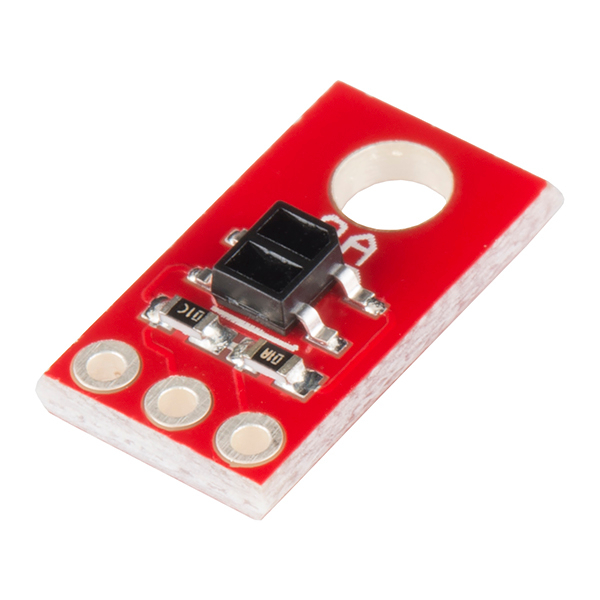
\includegraphics[width=0.7\textwidth]{figures/QRE.jpg}
	\caption{\text{Mounted QRE1113 sensor}}
	\label{Hardware diagram}
\end{figure}

%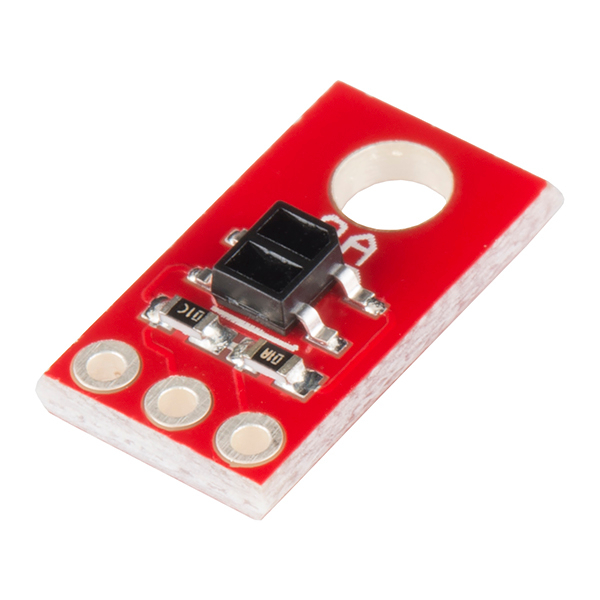
\includegraphics[width=0.7\textwidth]{figures/QRE.jpg}

\section{Analog-to-digital converter}


%\subsubsection{ADC diagram} 

%\includegraphics[width=0.7\textwidth]{figures/adcblock.PNG}


\subsubsection{The usage of ADC}
TBD (skal vi overhovedet forklare det igen? B: Vi skal nok forklare hvordan, og til hvad, vi udnytter det i projektet)

\section{The chipKIT Uno32 board}
The robot will utilize the chipKIT Uno 32 board to execute code. The board
was chosen both due to past experiences, but also because the robot would need
line-following properties, and we had already written a functional line-following robot
previously, which also included some important features, including PID control and 
pulse-width modulation patterns. \\
This enabled a lot of recycled code, which was a strong point
in the Uno 32's favor due to time constraints. \\

The board is also compatible with Arduino shields, and as such designing the H-bridge for it
becomes more straightforward. It's fast enough to execute the code, and works well within the
input power the robot will utilize.

\section{The motor shield}
The motor shield is containing the H-bridge and will be the board for ensuring control of the different components and motors.
TBD (hvad er der helt præcist på boarded?)

\subsection{The H bridge}
The robot will make use of an H-bridge. An H-bridge is a circuit made for controlling the motor of the robot, by making sure the motor will never try to do forward and backward motion  and cause errors or short circuits. The point of using an H-bridge is to ensure motor safety and functionality.

\subsection{The motors - Pololu}

\section{The Bluetooth tranceiver}
The robot will utilize the BlueSmiRF Silver bluetooth tranceiver. The transceiver is made by Sparkfun, it is utilized to make use of an GUI, by sending data from the MCU to the computer (GUI) by the use of bluetooth.\\ The bluetooth tranceiver makes it possible to monitor both the inputs and the logic behind the steering. The baudrate is between 2400-115200 bps and the tranceiver can be powered from 3.3v up to 6v. 

\section{Part conclusion}
After initial H-bridge problems, the rest of the process of building the robot went according to plan, and there were no future issues. The robot utillize a range of components which have been used for previous projects, which made the project much more simple to work with. This eliminated some of the learning curve that the previous robot presented, and made it possible to plan out and assemble the robot very rapidly, even though a lot of time was spent waiting for components for the motor shield, and the faulty components. This way, a lot more time could be used on programming and other software solutions. 
